% Title: gl2ps_renderer figure
% Creator: GL2PS 1.4.0, (C) 1999-2017 C. Geuzaine
% For: Octave
% CreationDate: Thu Nov 28 10:58:34 2019
\setlength{\unitlength}{1pt}
\begin{picture}(0,0)
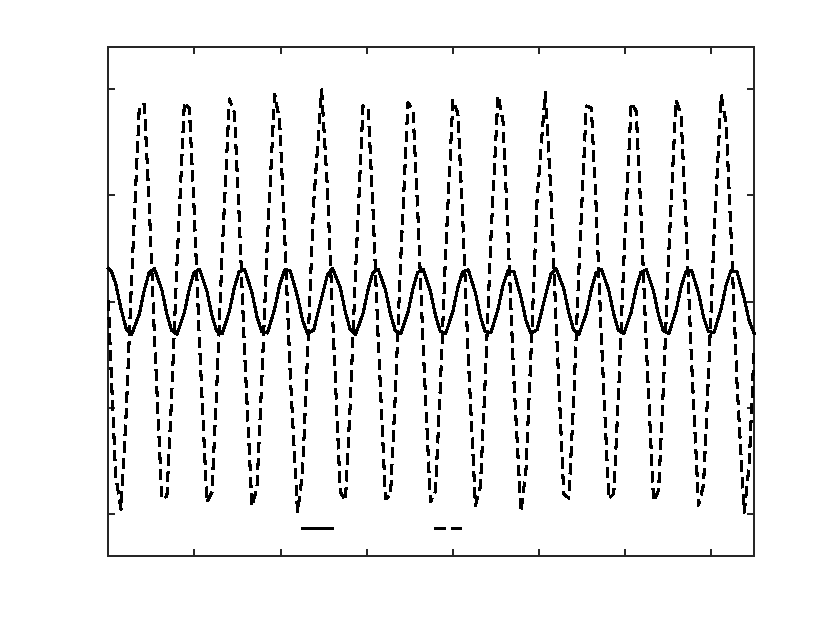
\includegraphics{../Report/img/PosVelNF-inc}
\end{picture}%
\begin{picture}(400,300)(0,0)
\fontsize{10}{0}
\selectfont\put(52,25.4846){\makebox(0,0)[t]{\textcolor[rgb]{0.15,0.15,0.15}{{0}}}}
\fontsize{10}{0}
\selectfont\put(93.3333,25.4846){\makebox(0,0)[t]{\textcolor[rgb]{0.15,0.15,0.15}{{2}}}}
\fontsize{10}{0}
\selectfont\put(134.667,25.4846){\makebox(0,0)[t]{\textcolor[rgb]{0.15,0.15,0.15}{{4}}}}
\fontsize{10}{0}
\selectfont\put(176,25.4846){\makebox(0,0)[t]{\textcolor[rgb]{0.15,0.15,0.15}{{6}}}}
\fontsize{10}{0}
\selectfont\put(217.333,25.4846){\makebox(0,0)[t]{\textcolor[rgb]{0.15,0.15,0.15}{{8}}}}
\fontsize{10}{0}
\selectfont\put(258.667,25.4846){\makebox(0,0)[t]{\textcolor[rgb]{0.15,0.15,0.15}{{10}}}}
\fontsize{10}{0}
\selectfont\put(300,25.4846){\makebox(0,0)[t]{\textcolor[rgb]{0.15,0.15,0.15}{{12}}}}
\fontsize{10}{0}
\selectfont\put(341.333,25.4846){\makebox(0,0)[t]{\textcolor[rgb]{0.15,0.15,0.15}{{14}}}}
\fontsize{10}{0}
\selectfont\put(47,53.375){\makebox(0,0)[r]{\textcolor[rgb]{0.15,0.15,0.15}{{-10}}}}
\fontsize{10}{0}
\selectfont\put(47,104.312){\makebox(0,0)[r]{\textcolor[rgb]{0.15,0.15,0.15}{{-5}}}}
\fontsize{10}{0}
\selectfont\put(47,155.25){\makebox(0,0)[r]{\textcolor[rgb]{0.15,0.15,0.15}{{0}}}}
\fontsize{10}{0}
\selectfont\put(47,206.188){\makebox(0,0)[r]{\textcolor[rgb]{0.15,0.15,0.15}{{5}}}}
\fontsize{10}{0}
\selectfont\put(47,257.125){\makebox(0,0)[r]{\textcolor[rgb]{0.15,0.15,0.15}{{10}}}}
\fontsize{11}{0}
\selectfont\put(207,12.4846){\makebox(0,0)[t]{\textcolor[rgb]{0.15,0.15,0.15}{{Tiempo}}}}
\fontsize{11}{0}
\selectfont\put(27,155.25){\rotatebox{90}{\makebox(0,0)[b]{\textcolor[rgb]{0.15,0.15,0.15}{{$\theta, \dot{\theta}$}}}}}
\fontsize{11}{0}
\selectfont\put(207,287.5){\makebox(0,0)[b]{\textcolor[rgb]{0,0,0}{{Posición y Velocidad del péndulo}}}}
\fontsize{9}{0}
\selectfont\put(161.918,46.1055){\makebox(0,0)[l]{\textcolor[rgb]{0,0,0}{{  $\theta$}}}}
\fontsize{9}{0}
\selectfont\put(225.75,46.1055){\makebox(0,0)[l]{\textcolor[rgb]{0,0,0}{{  $\dot{\theta}$}}}}
\end{picture}
